% Options for packages loaded elsewhere
\PassOptionsToPackage{unicode}{hyperref}
\PassOptionsToPackage{hyphens}{url}
%
\documentclass[
  man]{apa6}
\usepackage{amsmath,amssymb}
\usepackage{iftex}
\ifPDFTeX
  \usepackage[T1]{fontenc}
  \usepackage[utf8]{inputenc}
  \usepackage{textcomp} % provide euro and other symbols
\else % if luatex or xetex
  \usepackage{unicode-math} % this also loads fontspec
  \defaultfontfeatures{Scale=MatchLowercase}
  \defaultfontfeatures[\rmfamily]{Ligatures=TeX,Scale=1}
\fi
\usepackage{lmodern}
\ifPDFTeX\else
  % xetex/luatex font selection
\fi
% Use upquote if available, for straight quotes in verbatim environments
\IfFileExists{upquote.sty}{\usepackage{upquote}}{}
\IfFileExists{microtype.sty}{% use microtype if available
  \usepackage[]{microtype}
  \UseMicrotypeSet[protrusion]{basicmath} % disable protrusion for tt fonts
}{}
\makeatletter
\@ifundefined{KOMAClassName}{% if non-KOMA class
  \IfFileExists{parskip.sty}{%
    \usepackage{parskip}
  }{% else
    \setlength{\parindent}{0pt}
    \setlength{\parskip}{6pt plus 2pt minus 1pt}}
}{% if KOMA class
  \KOMAoptions{parskip=half}}
\makeatother
\usepackage{xcolor}
\usepackage{graphicx}
\makeatletter
\def\maxwidth{\ifdim\Gin@nat@width>\linewidth\linewidth\else\Gin@nat@width\fi}
\def\maxheight{\ifdim\Gin@nat@height>\textheight\textheight\else\Gin@nat@height\fi}
\makeatother
% Scale images if necessary, so that they will not overflow the page
% margins by default, and it is still possible to overwrite the defaults
% using explicit options in \includegraphics[width, height, ...]{}
\setkeys{Gin}{width=\maxwidth,height=\maxheight,keepaspectratio}
% Set default figure placement to htbp
\makeatletter
\def\fps@figure{htbp}
\makeatother
\setlength{\emergencystretch}{3em} % prevent overfull lines
\providecommand{\tightlist}{%
  \setlength{\itemsep}{0pt}\setlength{\parskip}{0pt}}
\setcounter{secnumdepth}{-\maxdimen} % remove section numbering
% Make \paragraph and \subparagraph free-standing
\ifx\paragraph\undefined\else
  \let\oldparagraph\paragraph
  \renewcommand{\paragraph}[1]{\oldparagraph{#1}\mbox{}}
\fi
\ifx\subparagraph\undefined\else
  \let\oldsubparagraph\subparagraph
  \renewcommand{\subparagraph}[1]{\oldsubparagraph{#1}\mbox{}}
\fi
\newlength{\cslhangindent}
\setlength{\cslhangindent}{1.5em}
\newlength{\csllabelwidth}
\setlength{\csllabelwidth}{3em}
\newlength{\cslentryspacingunit} % times entry-spacing
\setlength{\cslentryspacingunit}{\parskip}
\newenvironment{CSLReferences}[2] % #1 hanging-ident, #2 entry spacing
 {% don't indent paragraphs
  \setlength{\parindent}{0pt}
  % turn on hanging indent if param 1 is 1
  \ifodd #1
  \let\oldpar\par
  \def\par{\hangindent=\cslhangindent\oldpar}
  \fi
  % set entry spacing
  \setlength{\parskip}{#2\cslentryspacingunit}
 }%
 {}
\usepackage{calc}
\newcommand{\CSLBlock}[1]{#1\hfill\break}
\newcommand{\CSLLeftMargin}[1]{\parbox[t]{\csllabelwidth}{#1}}
\newcommand{\CSLRightInline}[1]{\parbox[t]{\linewidth - \csllabelwidth}{#1}\break}
\newcommand{\CSLIndent}[1]{\hspace{\cslhangindent}#1}
\ifLuaTeX
\usepackage[bidi=basic]{babel}
\else
\usepackage[bidi=default]{babel}
\fi
\babelprovide[main,import]{english}
% get rid of language-specific shorthands (see #6817):
\let\LanguageShortHands\languageshorthands
\def\languageshorthands#1{}
% Manuscript styling
\usepackage{upgreek}
\captionsetup{font=singlespacing,justification=justified}

% Table formatting
\usepackage{longtable}
\usepackage{lscape}
% \usepackage[counterclockwise]{rotating}   % Landscape page setup for large tables
\usepackage{multirow}		% Table styling
\usepackage{tabularx}		% Control Column width
\usepackage[flushleft]{threeparttable}	% Allows for three part tables with a specified notes section
\usepackage{threeparttablex}            % Lets threeparttable work with longtable

% Create new environments so endfloat can handle them
% \newenvironment{ltable}
%   {\begin{landscape}\centering\begin{threeparttable}}
%   {\end{threeparttable}\end{landscape}}
\newenvironment{lltable}{\begin{landscape}\centering\begin{ThreePartTable}}{\end{ThreePartTable}\end{landscape}}

% Enables adjusting longtable caption width to table width
% Solution found at http://golatex.de/longtable-mit-caption-so-breit-wie-die-tabelle-t15767.html
\makeatletter
\newcommand\LastLTentrywidth{1em}
\newlength\longtablewidth
\setlength{\longtablewidth}{1in}
\newcommand{\getlongtablewidth}{\begingroup \ifcsname LT@\roman{LT@tables}\endcsname \global\longtablewidth=0pt \renewcommand{\LT@entry}[2]{\global\advance\longtablewidth by ##2\relax\gdef\LastLTentrywidth{##2}}\@nameuse{LT@\roman{LT@tables}} \fi \endgroup}

% \setlength{\parindent}{0.5in}
% \setlength{\parskip}{0pt plus 0pt minus 0pt}

% Overwrite redefinition of paragraph and subparagraph by the default LaTeX template
% See https://github.com/crsh/papaja/issues/292
\makeatletter
\renewcommand{\paragraph}{\@startsection{paragraph}{4}{\parindent}%
  {0\baselineskip \@plus 0.2ex \@minus 0.2ex}%
  {-1em}%
  {\normalfont\normalsize\bfseries\itshape\typesectitle}}

\renewcommand{\subparagraph}[1]{\@startsection{subparagraph}{5}{1em}%
  {0\baselineskip \@plus 0.2ex \@minus 0.2ex}%
  {-\z@\relax}%
  {\normalfont\normalsize\itshape\hspace{\parindent}{#1}\textit{\addperi}}{\relax}}
\makeatother

% \usepackage{etoolbox}
\makeatletter
\patchcmd{\HyOrg@maketitle}
  {\section{\normalfont\normalsize\abstractname}}
  {\section*{\normalfont\normalsize\abstractname}}
  {}{\typeout{Failed to patch abstract.}}
\patchcmd{\HyOrg@maketitle}
  {\section{\protect\normalfont{\@title}}}
  {\section*{\protect\normalfont{\@title}}}
  {}{\typeout{Failed to patch title.}}
\makeatother

\usepackage{xpatch}
\makeatletter
\xapptocmd\appendix
  {\xapptocmd\section
    {\addcontentsline{toc}{section}{\appendixname\ifoneappendix\else~\theappendix\fi\\: #1}}
    {}{\InnerPatchFailed}%
  }
{}{\PatchFailed}
\keywords{systematicity, phonological development, preferential attachment, networks analysis\newline\indent Word count: FALSE}
\DeclareDelayedFloatFlavor{ThreePartTable}{table}
\DeclareDelayedFloatFlavor{lltable}{table}
\DeclareDelayedFloatFlavor*{longtable}{table}
\makeatletter
\renewcommand{\efloat@iwrite}[1]{\immediate\expandafter\protected@write\csname efloat@post#1\endcsname{}}
\makeatother
\usepackage{csquotes}
\usepackage[titles]{tocloft}
\cftpagenumbersoff{figure}
\renewcommand{\cftfigpresnum}{\itshape\figurename\enspace}
\renewcommand{\cftfigaftersnum}{.\space}
\setlength{\cftfigindent}{0pt}
\setlength{\cftafterloftitleskip}{0pt}
\settowidth{\cftfignumwidth}{Figure 10.\qquad}
\DeclareDelayedFloatFlavor{kableExtra}{table}
\usepackage{tipa}
\ifLuaTeX
  \usepackage{selnolig}  % disable illegal ligatures
\fi
\IfFileExists{bookmark.sty}{\usepackage{bookmark}}{\usepackage{hyperref}}
\IfFileExists{xurl.sty}{\usepackage{xurl}}{} % add URL line breaks if available
\urlstyle{same}
\hypersetup{
  pdftitle={Systematicity over the course of early development: an analysis of phonological networks},
  pdfauthor={Catherine E. Laing1},
  pdflang={en-EN},
  pdfkeywords={systematicity, phonological development, preferential attachment, networks analysis},
  hidelinks,
  pdfcreator={LaTeX via pandoc}}

\title{Systematicity over the course of early development: an analysis of phonological networks}
\author{Catherine E. Laing\textsuperscript{1}}
\date{}


\shorttitle{Systematicity and networks in early development}

\authornote{

All code and associated data for this manuscript can be found at \url{https://github.com/cathelaing/NetworkGraphs}. Data provided in the PhonBank corpus was collected through support from grant number NIH-NICHHD RO1-HD051698.

Correspondence concerning this article should be addressed to Catherine E. Laing, Department of Language and Linguistic Science, University of York, Heslington, YO10 5DD. E-mail: \href{mailto:catherine.laing@york.ac.uk}{\nolinkurl{catherine.laing@york.ac.uk}}

}

\affiliation{\vspace{0.5cm}\textsuperscript{1} University of York, York, UK}

\abstract{%
This paper explores the early lexicons of nine infants acquiring English or French to determine the extent of systematicity in the early vocabulary, and how this changes over time. Network graphs are generated from the point of first word production in the data set until age 30 months. Two measures of systematicity - mean path length and clustering coefficient - are analysed to establish the extent to which the early productive lexicon consists of closely-connected clusters of similar-sounding forms. Results show that early production is highly systematic when compared to random, prototypical and adult phonological networks, but that the network becomes more dispersed as it increases in size. Connectivity within the network is consistently higher for infants' actual productions when compared with the adult target forms, and this effect increases over time. This suggests a systematic approach to production over the course of early development.
}



\begin{document}
\maketitle

Infants' early words are phonologically similar to one another, if not in the vocabulary items they choose to produce, but in the way they produce them. This has been well-documented in a number of previous studies (e.g. Szreder, 2013; Vihman, 2016; Waterson, 1971), and can be clearly observed in datasets of early productions. For example, an inspection of Deuchar and Quay's (2000) record of their Spanish-English bilingual child's vocabulary acquisition shows that many of her earliest words are produced with an open CV syllable, and she produces a number of identical forms to refer to a range of different (though phonologically-similar) words. This suggests that infants may be drawing on a systematic approach to early productions, whereby a small subset of simple phonological forms are used to produce a range of more varied and phonologically-challenging adult targets. We would expect, therefore, that newly-acquired productions `cluster together' with existing forms, with high phonological similarity between new words and existing words in the lexicon. This paper will test this by analysing network graphs of the early vocabulary to determine how similar infants' words are to one another, and how this changes over time.

Network analysis is an increasingly popular method of analysing lexical acquisition, and offers an opportunity to consider production data on a larger scale than has previously been possible. Network models allow the analysis of connectivity within a system (in our case, the lexical or phonological system), and can track how that connectivity changes over time. In the case of language development, the nodes (individual items) in the network typically consist of words, and these are connected (or not) depending on how similar two nodes are in phonological or semantic space. Two words that are more similar to one another will be positioned closer together in the network, and less similar nodes further apart. Because this is a convenient way to think about language development over time, a number of studies have considered vocabulary acquisition within this framework. Analyses have considered infants acquiring their first language (e.g. Amatuni \& Bergelson, 2017; Fourtassi, Bian, \& Frank, 2020 ) and adults acquiring a novel language (e.g. Luef, 2022; Mak \& Twitchell, 2020; Siew \& Vitevitch, 2020).

Systematicity in early phonological development is most comprehensively discussed in work by Vihman and colleagues (e.g. Vihman, 2016, 2019; Vihman \& Croft, 2007; Vihman \& Keren-Portnoy, 2013). In more than four decades of work, incorporating data from a large number of infants acquiring an impressive range of languages, Vihman demonstrates a clear systematicity in infants' path to target-like word production. From the initial `surprisingly accurate' forms that appear in the first stages of word production, infants are shown to draw on what they know: they generally choose, for first production, words that are simple in their target phonological form, with consonants that are already familiar from the most common syllables of canonical babble (McCune \& Vihman, 2001). These forms are, in Vihman's terms, \emph{selected} for first word production owing to their easily-producible features. As the vocabulary grows, infant must necessarily acquire forms that do not contain such accessible phonological or segmental properties. Here we begin to see regression in the accuracy of early production, as infants systematically adapt forms to fit the most common structures and segments in their repertoire. When words are systematically altered to fit a dominant pattern in the child's output, these forms are said to be \emph{adapted}. Systematicity is apparent not just in the earliest words, but across the trajectory of acquisition as infants deal with the challenges of early word production by relying on well-rehearsed output forms. Over the first months of lexical development at least, infants' productions of newly-acquired words are likely to match their productions of existing words in the lexicon.

In recent work (Laing, under review), I draw on network analysis to analyse systematicity in the developing lexicon. I show that in the first three years of life, infants' production of new words can be predicted based on the words they already produce and how they produce them. That is, a word is more likely to be acquired if it is produced in a way that is phonologically similar to existing words in the productive repertoire, particularly when the new word is similar to a cluster of existing phonologically-similar forms in the output. This effect becomes stronger over time, suggesting that systematicity is more relevant to later word learning (at least, upto age 30 months) than in the first few months of word production. An analysis of target forms showed similar results, though with weaker predictive power. Moreover, the phonological properties of infants' word productions are more similar to one another than their adult target forms would suggest. These findings support the more fine-grained analyses presented by Vihman and colleagues, referenced above.

Other studies have used similar methods to test different kinds of data, to generate consistent (and some inconsistent) results. Laing (under review) drew on corpus data of fortnightly word production across nine infants; Kalinowski and colleagues (in prep) take a similar approach to Laing by analysing vocabulary norms from \textgreater1000 Norwegian infants taken longitudinally at up to six individual time-points. Their results also show evidence for systematicity in the target words acquired in early acquisition (the analysis of vocabulary norms means it is not possible to observe infant productions of these words). Systematicity was also identified in early word learning by Siew and Vitevitch (2020), in an analysis of vocabulary norms of children aged 3-9 years acquiring English and Dutch. Fourtassi and colleagues (2020), on the other hand, found no support for systematicity in their analysis of infants acquiring a range of 10 different languages, instead showing that salient properties of the input, rather than previously-learned phonological properties, predicted learning.

Note that the previous studies reported above (with the exception of Laing (under review)) all draw on vocabulary norming data, meaning that infants' actual productions (i.e.~the way they produce words) is not considered. One of the key strengths of Laing (under review) and the current paper is the application of phonological network analysis to real production data. From decades of work on early phonological development, we know that infants' earliest words are often far-removed, phonologically speaking, from their adult targets. For example Priestley's (1977) son is reported to produce \emph{banana} as /bajan/, \emph{sucker} as /fajak/, \emph{chocolate} as /kajak/ and \emph{medicine} as /mejas/ within the same week at age 1;10. The adult target forms are all highly variable in form, while the child forms all share the systematic implementation of a disyllabic production pattern with medial /j/, following the structure CVCVC. Such systematicity cannot even be hinted at from an analysis of the target forms only, thereby losing what may be a crucial aspect of the acquisition process. Moreover, Fourtassi and colleagues (2020) and Siew and Vitevitch (2020) draw on vocabulary norming data from a cross-sectional sample of infants, meaning it is only possible to take a very general view of acquisition, with no scope for considering individual variability across the sample. This work thus cannot address any questions about systematicity in early acquisition (though note that this was not the intention of either paper), but uses methods that have high potential for doing so.

All the previous work reported above uses network growth algorithms to test whether learning can be predicted based on the words that infants already know or produce. Such an approach can be used to test and/or compare different theoretical models of acquisition, whereby different network growth algorithms that index different predictions can be used as predictors in statistical models. This is a compelling computational approach to observing systematicity in the developing lexicon (as in Laing, under review), but does not give us a clear view into the extent to which early-acquired forms are produced in a phonologically similar way. That is, network growth models analyse connectivity (are two words similar, yes or no? if yes then they are connected in the network), rather than phonological distance (\emph{how} similar are two words in the network?). This study expands on previous work, and builds on findings from Laing (under review), by analysing network graphs of infants' early lexicons. This provides an insight into the properties of the network, including how densely-connected the network is, and the phonological distance between items in the network. It also allows us to make predictions about network properties over time that reflect word selection and adaptation, and thus presents an opportunity to apply Vihman's framework on a broader scale. Following Laing (under review), this paper will analyse infants' actual productions as well as the adult target forms, to test the extent to which systematicity is present in production, in terms of both the words infants select in early development, and how they produce them.

\hypertarget{research-questions-and-predictions}{%
\subsection{Research questions and predictions}\label{research-questions-and-predictions}}

This paper builds on previous network analyses by drawing on network graphs, instead of growth algorithms, to look more closely at the phonological distance between individual words in the developing lexicon. In doing so, it attempts to address the following questions:

\begin{enumerate}
\def\labelenumi{\arabic{enumi}.}
\tightlist
\item
  How systematic are early word productions, and (how) does this change over time?
\item
  Are the phases of word selection and adaptation identifiable in the dataset?
\end{enumerate}

To test these questions, network graphs will be generated using the \emph{igraph()} package (Csardi \& Nepusz, 2006) in R (R Core Team, 2020). To address the first question, properties of the graphs will be analysed to determine 1) how closely connected individual words are to one another; 2) how dense the overall distribution of words is in the network; and 3) how/whether this changes over time. Following Vihman's work, and findings presented by Laing (under review), it is expected that the early vocabulary will become increasingly systematic over time. This would be reflected in denser clusters of phonologically-similar forms and shorter distance between words. Simulated networks will be used to compare the real networks against both highly systematic and random networks to determine the extent of systematicity present in the data, and developmental changes over time.

To address the second question, network graphs of infants' actual productions will be compared with those of the target form, to trace the `target-likeness' of individual productions, and how this changes over time. Following Vihman once again, early word selection would be reflected in early similarities between Actual and Target network properties, as target forms are selected to match the structures and segments that infants are able to produce, meaning they should be produced with relative accuracy. Over time, Actual and Target forms are expected to diverge, such that Actual forms show more systematicity in the data than Target forms. Approaches used to test these predictions are outlined in detail below.

\hypertarget{methods}{%
\section{Methods}\label{methods}}

\hypertarget{data-extraction-and-preparation}{%
\subsection{Data extraction and preparation}\label{data-extraction-and-preparation}}

This study draws on the same data as that analysed by Laing (under review). This was drawn from two corpora on PhonBank (Rose \& MacWhinney, 2014): Providence (American English - Demuth, Culbertson, \& Alter, 2006) and Lyon (French - Demuth \& Tremblay, 2008). These were selected due to their equivalent data collection methods and the fact that the infants' productions, as well as the corresponding target forms, are phonetically transcribed. Nine infants' (5 English, 4 French, 4 boys overall) data were extracted using Phon (Hedlund \& Rose, 2020), from the transcript with their first-recorded word to the final transcript taken at age 2;6. Infants were recorded in the home on a fortnightly basis, participating in naturalistic interactions with their caregivers. Two of the American infants were recorded weekly during some periods of data collection, but this is not an issue for this analysis since no between-child comparisons will be made. See Demuth et al. (2006) and Demuth and Tremblay (2008) for full details of data collection.

Extracted data was filtered to include only words featuring on the communicative development inventory (CDI) of the respective language, including all variants of a given form (including a total of 680 possible word types for American English and 690 for European French). For example, plurals were included alongside the singular noun form, and variable verb conjugations alongside their corresponding infinitive verb form. These data were used to create a network for each infant for each month of data, whereby all words in a given month that hadn't been produced in previous months were included as new items in the network. When a word had been produced in previous months, it was not included. While this means that the data does not capture change in the production of a single form over time, it allows us to observe network growth at the point of acquisition for each word form.

To determine the structure of the network, the first step was to create distance values between each word and each other word in the network. This was first done using a `global' network of all forms produced by the infant up to the final session at 2;6, to create a large distance matrix for each infant that incorporated all word productions. Essentially, this global network reflects the distance between every word and every other word in each child's productive vocabulary at 2;6. Distance values were established using methods set out in Monaghan et al. (2010), using distinctive features to generate a set of phonetic values for each word that could then be compared with all other words (note that only consonants were analysed, given that vowels are highly variable in early production and also very difficult to transcribe accurately, Donegan, 2013; Kent \& Rountrey, 2020). Euclidean distance between the values of each word and each other word in each infant's global network was then used to determine how close/distant words were from one another. Often, infants produced multiple tokens of the same word type in a given month, often with high variability across tokens. Because it was not possible to generate networks with all tokens included (even with only single word types included, the final dataset for all nine infants includes over 5.5 million data points, once distance between each word and each other word is calculated), a mean value for each distinctive feature was established across tokens, meaning that each word's distinctive feature value represents the variability of the infant's production of a given word. This may not be a perfect measure, but it is more representative than taking, for example, the first instance of each word type.

Distance scores were generated between each word and each other word in each child's dataset, for both Target and Actual forms. These scores were then normalised, and a normalised distance of 0.25 was chosen to indicate connectivity. That is, words were said to be connected in the network if their distance score was 0.25 or less. This accounted for the lower quartile of connectivity across the dataset. See Supplementary Materials (S1) for an overview of how this measure was established.

The final dataset includes 3223 word types in total, with 1927 in the English corpus and 1296 in the French corpus. On average, infants produced 47 tokens of each word type in a single session (SD = 170; mean English tokens = 40, SD = 143; mean French tokens = 58, SD = 202).

\hypertarget{data-analysis}{%
\subsection{Data analysis}\label{data-analysis}}

\hypertarget{network-graphs}{%
\subsubsection{Network graphs}\label{network-graphs}}

The prepared data was then used to generate a series of network graphs for each infant (for both Target and Actual data) using the \emph{igraph()} package in R (Csardi \& Nepusz, 2006). One network was generated per month, for each month in the dataset, based on all words produced in the given month and all months prior. The network at time-point \emph{n}+1 thus included all words produced upto and including time-point \emph{n}, plus all additional words produced for the first time at \emph{n}+1. The \emph{igraph()} package generates graphs that include all nodes (whether or not they are connected to other nodes\footnote{Recall that any two nodes that have a scaled phonological distance of \textgreater.25 will not be connected.}), and measures the distance between all connected nodes, as well as the clustering of nodes in graphical space.

Two key variables will be explored through an analysis of network graphs: \emph{mean path length} and \emph{average clustering coefficient}. Path length is a measure of distance between nodes, and mean path length indexes the average phonological distance (of all connected nodes) within a network; by this measure, we would expect that systematicity in early phonological development would be reflected in \emph{low} mean path length. Clustering coefficient is an indication of network density: a \emph{higher} average density of nodes in the network indicates denser clusters of similar forms; again, this is what we would expect to see in a network of early phonological development. See Goldbeck (2013) for a full overview of network structures and measures.

\hypertarget{simulated-networks}{%
\subsubsection{Simulated networks}\label{simulated-networks}}

Networks with high phonological systematicity should exhibit properties of prototypical ``small-world'' network growth, namely a low mean path length and a high average clustering coefficient (Amaral, Scala, Barthelemy, \& Stanley, 2011; Steyvers \& Tenenbaum, 2005; Watts \& Strogatz, 1998). Words should be more densely connected, with shorter connections between words. As this is what we expect to see in the phonological networks tested here, small-world networks serve as a suitable comparison with the real data. If high systematicity is present in the data, then there should be no statistical difference between the real network and a small-world network of equal size. To test this, mean path length and clustering coefficient values were generated for both the Target and Actual networks, as described above. Data were then compared to the growth of a simulated small-world network of equal size, known as a Watts-Strogatz network (Watts \& Strogatz, 1998). This network was generated computationally in R using the \emph{igraph()} package (Csardi \& Nepusz, 2006), and was matched for network size and mean connectivity within the network at each month. The real data were also compared to a similarly-sized but randomly-generated network known as a Erdős--Rényi model. If the real network grows in a systematic way, then we would expect the real data to differ significantly from the randomly-generated Erdős--Rényi network. Again, this was generated using the \emph{igraph()} package (Csardi \& Nepusz, 2006), and was matched for network size at each month (but not mean connectivity, as this is not required for a random graph). To run these analyses, mean path length and clustering coefficient were calculated for each monthly graph - the Real data, and the two kinds of simulated data (prototypical systematic network vs.~random network) - and the two kinds of Simulated network were tested against the Real network.

\hypertarget{results}{%
\section{Results}\label{results}}

\hypertarget{rq1-how-systematic-are-early-word-productions-and-how-does-this-change-over-time}{%
\subsection{RQ1: How systematic are early word productions, and (how) does this change over time?}\label{rq1-how-systematic-are-early-word-productions-and-how-does-this-change-over-time}}

To test RQ1, network graphs were compared to simulated small world and random networks of equivalent size to determine whether the data (the \emph{Real} network, drawing from infants' Actual productions) differed from the \emph{Simulated} networks. For both mean path length and clustering coefficient, we would expect the Real data to differ significantly from the Simulated Erdős--Rényi (random) network, and for the Real network to show similar properties to the Simulated Watts-Strogatz (small-world) network. Note that the extent of the expected statistical difference is not easy to predict here: if the Real network is very similar to the Watts-Strogatz network then no statistical difference would be expected, but this relies on the Real data being highly systematic, which may not be realistic. In order to fully understand the nature of the data, figures and model outputs will be inspected in relation to these predictions.

The two measures will be discussed in turn. Models include mean path length or average clustering coefficient as the dependent variable, respectively, each with data type (Real vs.~small-world vs.~random), corpus (English vs.~French) and age as fixed effects, and subject as a random effect with a by-Subject random slope for the effect of age. Initial model comparisons showed that including network size, alongside age, improved fit in the model testing clustering coefficient, but not mean path length (see S2). Network size is thus included as a fixed effect in the clustering coefficient model only.

\hypertarget{mean-path-length}{%
\subsubsection{Mean Path Length}\label{mean-path-length}}

\begin{figure}
\centering
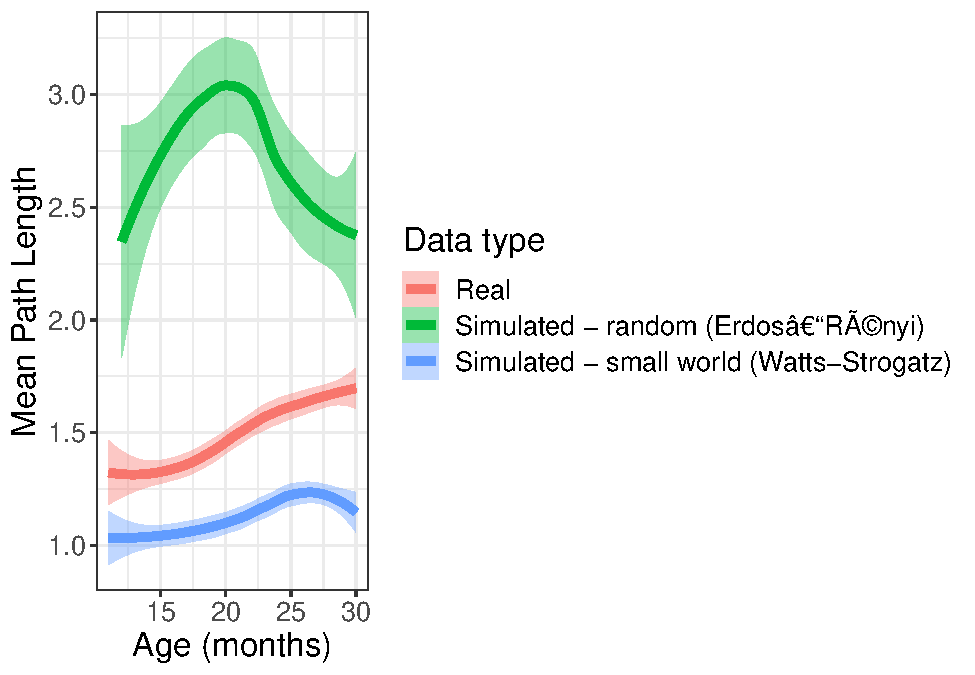
\includegraphics{NetworkGraphs_files/figure-latex/Figure-path-length-1.pdf}
\caption{\label{fig:Figure-path-length}Change in mean path length as network size increases, in Real vs.~Simulated (random and small-world) data. Coloured lines represent Data type; coloured bands represent 95\% CIs.}
\end{figure}

Nested model comparisons revealed a significant effect for Data type on mean path length. See Table \ref{tab:table-model-output}. As shown in Table \ref{tab:table-real-sim}, the Real data had a significantly lower mean path length than the random Simulated data, as predicted. The difference between the Real data and the Simulated small world data was also significant, but the extent of this difference was smaller than for the comparison with the random network. The extent of these effects is shown clearly in Figure \ref{fig:Figure-path-length}, where the comparison between the Real data and the random Simulated data is visually much wider than that of the Real vs.~Simulated small-world network. Contrary to predictions, there was no change in systematicity over time (i.e.~no effect of Age was observed).

\begin{figure}
\centering
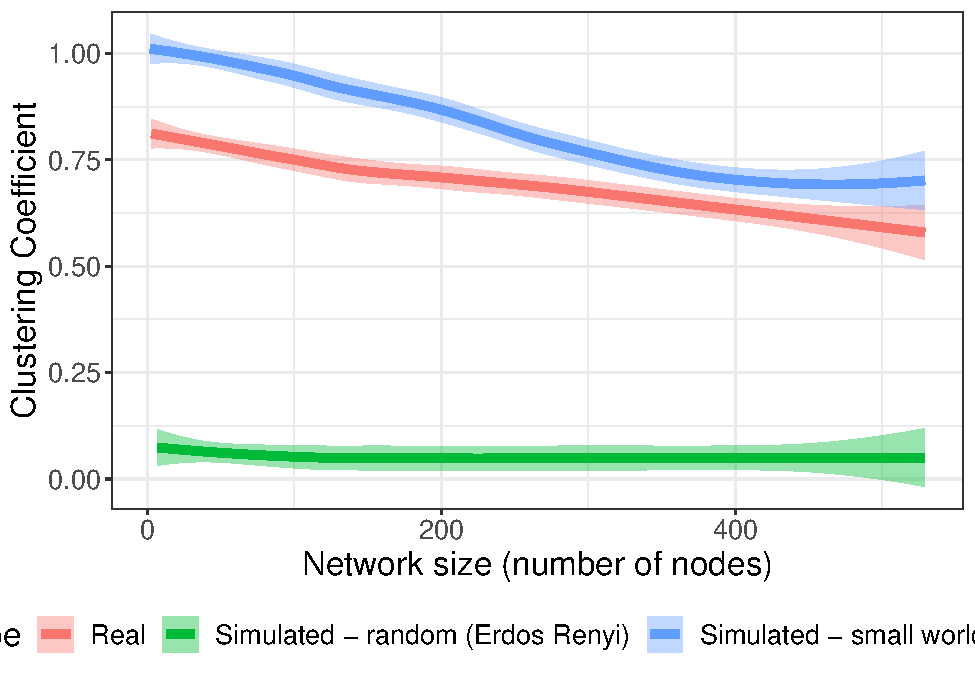
\includegraphics{NetworkGraphs_files/figure-latex/Figure-clust-coef-1.pdf}
\caption{\label{fig:Figure-clust-coef}Change in mean path length as network size increases, in Real vs.~Simulated (random and small-world) data. Coloured lines represent Data type; coloured bands represent 95\% CIs.}
\end{figure}

\hypertarget{clustering-coefficient}{%
\subsubsection{Clustering coefficient}\label{clustering-coefficient}}

The same main outcomes were found when clustering coefficient was tested in the model. See Tables \ref{tab:table-model-output} and \ref{tab:table-real-sim}. The Real data had a significantly higher clustering coefficient than the random Simulated data, but this was significantly lower than that of the small-world Simulated data. Again, the magnitude of the difference was much larger in the Real vs.~random Simulated comparison than the Real vs.~small world Simulated comparison. This is visualised clearly in Figure \ref{fig:Figure-clust-coef}. Again there was no effect for Corpus on the data, but this time there was a significant effect for Age: clustering coefficient values increased over time, suggesting that systematicity became stronger in the data over time; with each additional month, clustering coefficient increased by 0.40\%. However, a significant effect for network size contradicts this; with each additional word added to the network, clustering coefficient decreased by 0.10\%.

\hypertarget{actual-vs.-target-data}{%
\subsubsection{Actual vs.~Target data}\label{actual-vs.-target-data}}

The differences between the Real data and the small-world Simulated data are difficult to interpret, given that there is no clear model of what phonological systematicity would look like in a highly systematic small-world network. To further interrogate systematicity within the data, network properties of the Real (Actual) data analysed above were compared to the Real Target data. Target data serves as an appropriate proxy for connectivity and clustering within a ``standard'' phonological network, albeit a network that is constrained by words produced in early acquisition, and further constrained by the fact that only a subset of these (i.e.~CDI words) are included in the data set. We would expect that mean path length and clustering coefficient would each show higher systematicity in the Actual network than the Target network\footnote{Note that this result was observed for network growth models in Laing (under review), whereby the Actual network was found to be a better predictor of learning based on the known network of each child.}. Basic model structure was the same as reported above, but with only Real data (Actual vs.~Target) considered as a fixed effect. The inclusion of network size as a fixed effect improved model fit for both dependent variables and so was included in both models.

There was a significant effect for Data type on mean path length. See Table \ref{tab:table-model-output}. Model outputs revealed that Target data had a significantly higher mean path length than Actual data (see Table \ref{tab:table-actual-target} and Figure \ref{fig:Figure-path-length-DT}. This time there was a significant effect for Corpus, whereby the French data had a higher mean path length than the English data overall. Network size, but not Age, significantly affected mean path length, which increased as Network size increased, indicating a decrease in systematicity over time: with each new word added to the network, mean path length decreased by 0.10\%.

The effect of Data type on clustering coefficient was also significant. Mean clustering coefficient was significantly lower in Target compared with Actual data. See Figure \ref{fig:Figure-clust-coef-DT}. The French data had a significantly lower mean clustering coefficient than the English data. Again, there was a significant effect for Network size, and this was consistent with the result reported above for mean path length, in that it indicated a decrease in systematicity with increased network size. As new words were acquired in the network, mean clustering coefficient decreased by 0.05\%. Here, Age was not a significant predictor of changes in clustering coefficient.

\begin{longtable}[t]{cccc}
\caption{\label{tab:table-model-output}Outputs from nested model comparisons testing the effect of data type (Real vs. Simulated and Actual vs. Target on mean path length and clustering coefficient.}\\
\toprule
Model & Df & Chisq & p\\
\midrule
Mean Path Length (Real vs. Simulated) & 2 & 525.39 & <0.001\\
Mean Path Length (Actual vs. Target) & 1 & 359.58 & <0.001\\
Clustering Coefficient (Real vs. Simulated) & 2 & 1176.40 & <0.001\\
Clustering Coefficient (Actual vs. Target) & 1 & 124.47 & <0.001\\
Mean connectivity (Actual vs. Target): GAMM & 3 & 173.71 & <0.001\\
\bottomrule
\end{longtable}

\begin{longtable}[t]{ccccccccc}
\caption{\label{tab:table-real-sim}Outputs from linear regression models testing comparisons of Real vs. Simulated data on mean path length and clustering coefficient.}\\
\toprule
\multicolumn{1}{c}{ } & \multicolumn{4}{c}{Mean path length} & \multicolumn{4}{c}{Clustering coefficient} \\
\cmidrule(l{3pt}r{3pt}){2-5} \cmidrule(l{3pt}r{3pt}){6-9}
Effect & beta & SE & t & p & beta & SE & t & p\\
\midrule
Intercept & 1.350 & 0.12 & 11.225 & <0.001 & 0.747 & 0.02 & 29.924 & <0.001\\
Real vs. Erdos–Rényi & 1.210 & 0.05 & 23.605 & <0.001 & -0.666 & 0.01 & -60.302 & <0.001\\
Real vs. Watts-Strogatz & -0.373 & 0.05 & -7.454 & <0.001 & 0.159 & 0.01 & 14.745 & <0.001\\
Corpus & 0.032 & 0.04 & 0.725 & 0.471 & -0.014 & 0.01 & -1.292 & 0.225\\
Age & 0.007 & 0.00 & 1.343 & 0.213 & 0.004 & 0.00 & 2.746 & 0.009\\
\addlinespace
Network size & NA & NA & NA & NA & -0.001 & 0.00 & -11.128 & <0.001\\
\bottomrule
\end{longtable}

\begin{longtable}[t]{ccccccccc}
\caption{\label{tab:table-actual-target}Outputs from linear regression models testing comparisons of Actual vs. Target data on mean path length and clustering coefficient.}\\
\toprule
\multicolumn{1}{c}{ } & \multicolumn{4}{c}{Mean path length} & \multicolumn{4}{c}{Clustering coefficient} \\
\cmidrule(l{3pt}r{3pt}){2-5} \cmidrule(l{3pt}r{3pt}){6-9}
Effect & beta & SE & t & p & beta & SE & t & p\\
\midrule
Intercept & 1.166 & 0.08 & 15.350 & <0.001 & 0.8804 & 0.03 & 30.079 & <0.001\\
Actual vs. Target & 0.300 & 0.01 & 27.072 & <0.001 & -0.1022 & 0.01 & -12.481 & <0.001\\
Corpus & 0.068 & 0.02 & 3.644 & 0.006 & -0.0425 & 0.01 & -4.682 & <0.001\\
Age & 0.004 & 0.00 & 1.083 & 0.294 & -0.0023 & 0.00 & -1.613 & 0.121\\
Network size & 0.001 & 0.00 & 17.232 & <0.001 & -0.0005 & 0.00 & -11.915 & <0.001\\
\bottomrule
\end{longtable}

\begin{figure}
\centering
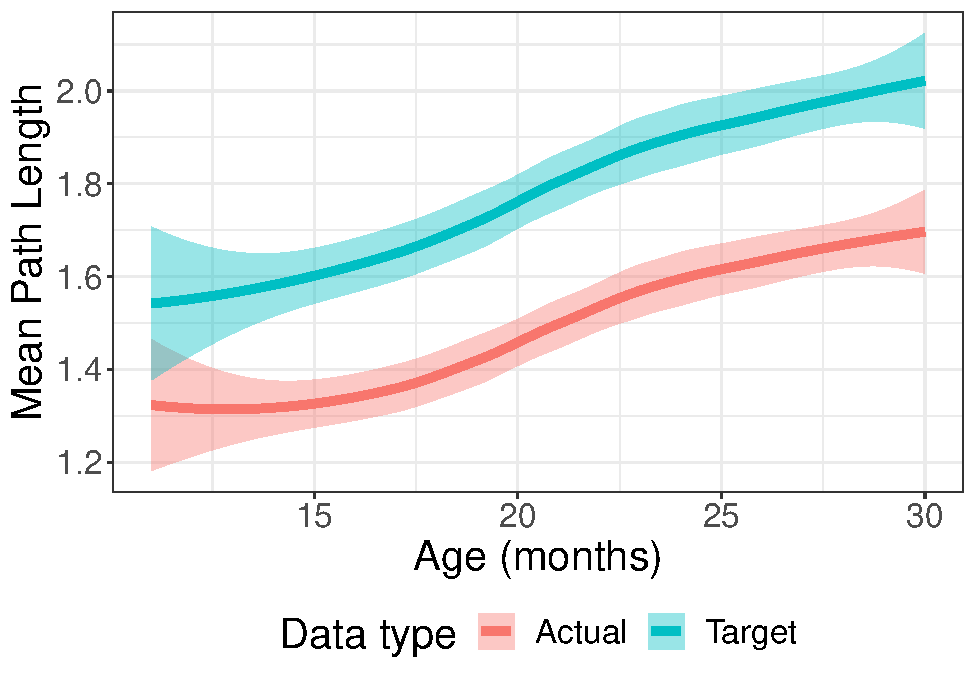
\includegraphics{NetworkGraphs_files/figure-latex/Figure-path-length-DT-1.pdf}
\caption{\label{fig:Figure-path-length-DT}Change in mean path length as network size increases, in Actual vs.~Target data. Coloured lines represent Data type; coloured bands represent 95\% CIs.}
\end{figure}

\begin{figure}
\centering
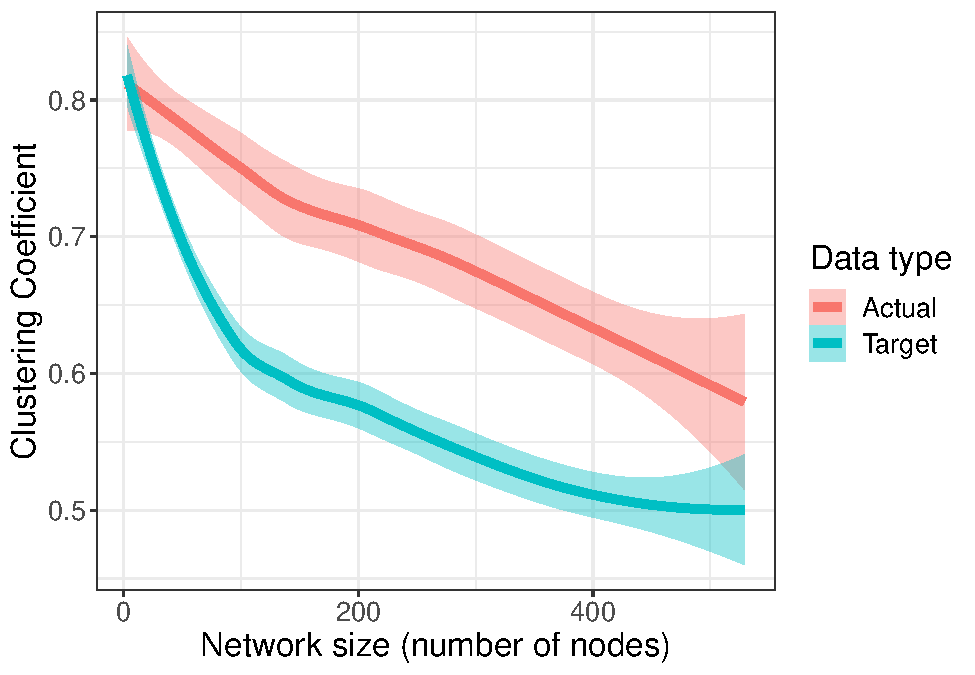
\includegraphics{NetworkGraphs_files/figure-latex/Figure-clust-coef-DT-1.pdf}
\caption{\label{fig:Figure-clust-coef-DT}Change in mean clustering coefficient as network size increases, in Actual vs.~Target data. Coloured lines represent Data type; coloured bands represent 95\% CIs.}
\end{figure}

\hypertarget{rq2.-is-there-evidence-of-word-selection-and-adaptation-in-the-dataset}{%
\subsection{RQ2. Is there evidence of word selection and adaptation in the dataset?}\label{rq2.-is-there-evidence-of-word-selection-and-adaptation-in-the-dataset}}

To address the second research question, the phonological distance between Target and Actual forms was taken as a proxy of word selection and adaptation. That is, if a word is produced in a target-like way (i.e.~assumed to be selected\footnote{though note that, while a selected form is, by definition, target-like in phonological form, a target-like form isn't necessarily a selected form.}), then the phonological distance between the Target form and the way it is produced (Actual form) should be low. The opposite is true for adapted forms, as we expect, by definition, a non-target-like production and thus a higher distance between Target and Actual form. This measure is not perfect, but coding selected/adapted forms would otherwise have to be done by hand, which is not feasible across such a large dataset. Following Vihman's (2019) framework, we would expect low distance been Actual and Target forms earlier on in development as words are selected, and higher distance later as word adaptation begins to take hold. To test this, I drew on generalised additive mixed effects models (GAMMs), since these allow the analysis of non-linear change over time, and can account for statistical differences between two non-linear trajectories of data that may differ in non-linear ways (Sóskuthy, 2017; Wieling, 2018).

First, GAMMs were used to examine connectivity of the infants' Actual and Target networks and how these changed over time. These were run using the \emph{mgcv()} package in R (Wood, 2011). These models analyse the extent to which the two networks differ (or not) from one another across infants, and how this changes non-linearly month-by-month. Fixed effects in the model can include parametric terms, as is typical in regression modelling, and also \emph{smooth terms}, or non-linear fixed effects. Much like mixed-effects linear models, GAMMs can account for random effects in the data; in this case by-subject random effects were included through the addition of \emph{random smooths} in the model.

The model tested mean number of connections in the network (average number of connections of each node in the network, or \emph{mean k}) as the dependent variable, working on the assumption that connectivity in the Target vs.~Actual networks would be similar during periods of word selection (i.e.~Actual and Target words are similar to one another and so distribution of connectivity should be similar), and would differ during periods of adaptation. Specifically, periods of adaptation should lead to higher connectivity in the Actual network than the Target network, since we expect productions to be more similar (and thus more well-connected) in Actual forms; we would expect connectivity across data types to diverge at the point that word adaptation begins to take hold. A higher number of connections (higher mean k) for Actual vs.~Target networks is expected during periods of adaptation, and no difference in connectivity is expected for periods of selection. Data type (Actual vs.~Target) and corpus (English vs.~French) were included as parametric terms, with Data type being the variable of interest in the model. Network size and Age were included as smooth terms, as well as by-Subject and by-Data type random smooths for the effect of Age, which account for by-Subject and by-Data type differences in the data over time.

To account for the fact that adjacent values (i.e.~connectivity at month \emph{n} and month \emph{n+1}) are likely correlated, GAMM modelling includes an autocorrelation parameter; see Sóskuthy (2017) and Wieling (2018) for full details. Additionally, the start point for each infant's data (i.e.~their first recording session) was indexed in the model. To test for an effect of Data type, model comparisons were run using the \emph{compareML()} function from the \emph{itsadug()} package (Rij, Wieling, Baayen, \& Rijn, 2022): the full model including the effect of Data type and the by-Data type random smooth was compared to a model without these terms. Because model summaries for GAMM smooths may be non-conservative (\emph{Sóskuthy, 2017}), smooth plots will be observed alongside any significant effects to determine relevant trends in the data.

Model comparisons revealed a significant effect for Data type on connectivity in the networks over time. See Table \ref{tab:table-GAMM-outputs}. Figure \ref{fig:difference-plot-mean-k} shows the difference between Actual and Target connectivity over the course of development. The red line indicates periods of significant difference, showing that Actual vs.~Target connectivity was significantly different throughout the period of analysis; Actual forms were always more well-connected than Target forms. This contrasts with the expectations set out above. However, Figure \ref{fig:difference-plot-mean-k} clearly shows an increase in the difference in connectivity between Actual and Target forms over the period of data collection, supporting the expectation that Target and Actual forms are more similar earlier on in development, with an increasing difference in mean connectivity over the course of the analysis, favouring higher connectivity in Actual, compared with Target, forms.

\begin{figure}
\centering
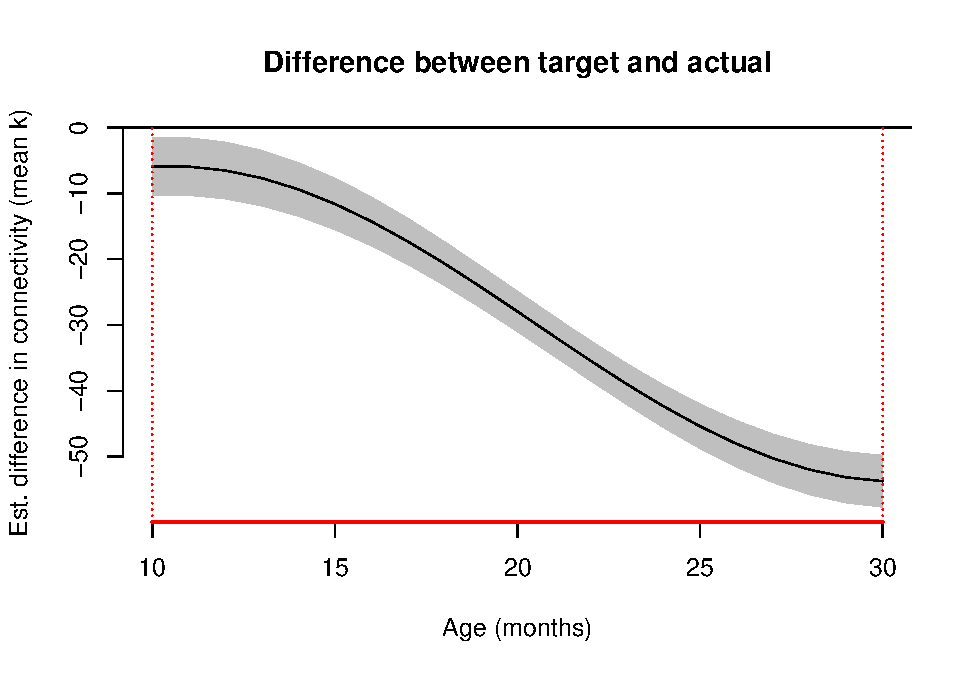
\includegraphics{NetworkGraphs_files/figure-latex/difference-plot-mean-k-1.pdf}
\caption{\label{fig:difference-plot-mean-k}Difference smooth plot showing difference between connectivity (mean k) in Actual vs.~Target forms from the GAMM model specified above. Shaded area shows 95\% confidence intervals, red line along x-axis indicates months in which
the difference between Actual and Target forms was significant.}
\end{figure}

\hypertarget{discussion}{%
\section{Discussion}\label{discussion}}

This paper set out to test the presence of systematicity in infants' developing lexicons by analysing phonological network graphs from nine infants acquiring French or English. Network graphs allow a close-up view of phonological similarity between forms within the network (via mean path length) and the extent to which groups of phonologically similar forms cluster together (via average clustering coefficient). Systematicity in the network would be reflected in shorter distance between forms and higher clusters of phonologically similar forms. The analysis also sought to identify periods of selection and, later, adaption - indicating a shift towards increasing systematization - in the data.

The first research question asked whether or not systematicity could be identified using a network graphs analysis, and, if so, whether or not this changed over time. This essentially presents a replication of questions tested on the same data by Laing (under review), using a different analytical approach. Comparisons of network graphs generated using the real data against random and highly systemtatic simulated network graphs lent support towards the presence of systematicity within the data, and this was strengthened with a follow-up analysis comparing networks of the infants' actual productions with those of the target forms. Overall, infants' early productions were closer in phonological distance (mean path length) and formed denser clusters of similar forms within the networks (average clustering coefficient) than simulated random networks and networks of the target phonological forms, though these were less systematic than prototypical highly systematic ``small world'' simulated networks. These findings support those of Laing (under review) to show that systematicity is present in early phonological productions.

The picture gets a little more complex when changes over time are considered. Laing (under review) identified an increase in the predictive power of the network model over time, which indicated increasing systematicity in the network. However, this was not the case for the present analysis, and in fact the opposite was true overall. Mean path length was not affected by changes in age, but it did increase with network size, at least in the model testing only Real (Actual vs.~Target) data (note that this variable was not included in the model testing the Real vs.~Simulated data). The observed increase in mean path length indicates \emph{decreasing} systematicity, as nodes are increasingly more widely-dispersed across the network. This is opposite to what was expected. The findings for clustering coefficient were a little more mixed, but point to similar trends overall. In the Real vs.~Simulated analysis, both age and network size predicted changes in clustering coefficient, but in opposite directions; as network size increased, clustering coefficient decreased, yet this measure increased with increasing age. In the model testing Actual vs.~Target data (the model that best reflected a realistic learning scenario), only network size predicted learning, and this was again in favour of \emph{decreasing} systematicity: as network size increased, clustering coefficient decreased.

The second research question attempted to identify periods of word selection and adaption in the data using generalised additive mixed models (GAMMs). This analysis worked on the assumption that overall connectivity in the network (mean number of connections per node, or \emph{mean k}) should be similar for Actual and Target forms during periods of word selection, since infant productions should be more phonologically accurate for selected words, and thus similar in connectivity to the target forms. Periods of adaptation, on the other hand, should see a difference in connectivity between Target and Actual data; new target forms in the network will be more distant, and less likely to connect to existing forms, whereas actual forms should continue to connect to existing words in the network. Thus, we expect a divergence between connectivity in the Target and Actual networks. This was, to some extent, borne out in the data, though distinct periods of selection and adaptation could not be identified. Instead, a gradual increase in the difference in connectivity between Actual and Target networks was observed over time; the difference in connectivity was always significant, and mean k was always higher in Actual than Target networks.

The first question to address regarding the present analysis is how these results compare to those of Laing (under review), since both similarities and inconsistencies were identified across the two methods. The consistency in evidence for systematicity in the data, in particular in the Actual forms, lends strong support towards the argument for a reliance on a ``phonic core of remembered lexical items and articulations'' (Ferguson \& Farwell, 1975, p. 112) in development, which are systematically drawn upon to tackle the challenges of remembering and producing early words. Across these two studies, four different analysis methods {[}network growth models and GAMMs testing network growth in Laing (under review); network graph analysis and GAMMs testing connectivity in the present study{]} have shown consistent and statistically-supported evidence for systematicity. On the other hand, a key difference across the results is the contradictory findings regarding change over time.\footnote{Note that the variables showing this trend differed across studies: Laing (under review) found an increase in systematicity as infants got older, whereas here age was not a predictor of changes in our variables, while network size revealed a decrease in systematicity.} However, to address this we might consider what it would mean for these two variables to change in the opposite direction over time (i.e.~indicating an increase in systematicity). Decreasing mean path length would mean that words are becoming more similar to one another, and increasing clustering coefficient would indicate denser clusters of these increasingly similar forms. In developmental terms, this would not be a sustainable method of increasing vocabulary; as new words are produced, we would expect the network to become more dispersed over time, with an increasing number of clusters that likely increase in their variability (and are thus less densely-connected). For efficient and realistic word learning, it seems there is no direction for these two variables to go but up/down, respectively, as we see in the data. Indeed, this outcome aligns well with care study accounts of infants' early words, where we see the establishment of different production patterns, or templates (Vihman, 2019) over time, for example Waterson's (1971) case study of her son's production, where five distinct systematic structures are identified in his data. Note that when we observe connectivity in the network with GAMMs, we see age-related changes in the expected direction (see Figure \ref{fig:difference-plot-mean-k}).

The second question arising from these findings is the extent to which network graphs - in particular the measures used in this study - can help us understand systematicity. Even though this analysis incorporated a more close-up analysis of network properties than those that draw on network growth models alone by taking into account distribution of the nodes within the networks across three measures (mean path length, average clustering coefficient, and mean k), still the analyses all abstract away from the detail of early word production, and specifically what drives connectivity and clustering within the network. The measures used to generate phonological distance were not able to take into account holistic or prosodic properties of early words, so we lose a potential source of connectivity within infants' early words (for example, a reliance on consonant harmony, which reveals within-word, as well as potential between-word, systematicity). Kalinowski and colleagues (in prep) take steps towards addressing this in their analysis, showing the potential for even more nuanced indices of phonological distance. Moreover, infants are likely to have drawn on different approaches to early word production, some which might have been represented as systematic more effectively by the measures used here. Finally, the focus on mean k to analyse word selection and adaptation is likely a crude measure for changes in the data that are likely very subtle. Future work may want to draw on cluster analysis to observe these changes in the data more closely. That being said, phonological distance between Target and Actual forms may be a useful measure for objectively identifying word selection or adaptation in future studies.

While this analysis presents a more nuanced view of systematicity than in previous studies that draw entirely on network growth models, including Laing (under review), Fourtassi and colleagues (2020) and Siew and Vitevitch (2020), closer inspection of the network graphs themselves may have been useful in supporting and explaining the findings in more detail. Future work could combine computational analyses of networks with a more impressionistic analysis of infants' early word productions to bring together these two very different but equally valuable methodologies. Indeed, drawing on modelling to understand large-scale data makes it possible to quantify findings in a more rigorous way, but it abstracts away for the nature of early productions and means we miss out on the detail of the patterns that are being drawn upon. It also overlooks the extent to which infants take very individualised paths in phonological development (Vihman, 1993), and the possibility that broad-scale generalization is simply not reflective of the reality of early production.

Overall, these findings support a case for systematicity in early development. The analysis of network graphs supports and builds on existing studies in this area - those that present a `close-up' case-study analysis (e.g. Szreder, 2013; Waterson, 1971) and those that draw on computational methods to analyse large data sets in a generalised way (e.g. Fourtassi et al., 2020; Laing, under review) - to present a nuanced evaluation of a large-scale early production data set. Findings suggest that the developing network is characterised by an increasing number of dense clusters of similar-sounding words, and that systematicity is present in early production from the beginning.

\hypertarget{refs}{}
\begin{CSLReferences}{1}{0}
\leavevmode\vadjust pre{\hypertarget{ref-amaral_classes_2011}{}}%
Amaral, L. A. N., Scala, A., Barthelemy, M., \& Stanley, H. E. (2011). Classes of small-world networks. In \emph{The structure and dynamics of networks} (pp. 207--210). Princeton, {NJ}: Princeton University Press.

\leavevmode\vadjust pre{\hypertarget{ref-amatuni_semantic_2017}{}}%
Amatuni, A., \& Bergelson, E. (2017). \emph{Semantic {Networks} {Generated} from {Early} {Linguistic} {Input}} {[}Preprint{]}. \url{https://doi.org/10.1101/157701}

\leavevmode\vadjust pre{\hypertarget{ref-R-igraph}{}}%
Csardi, G., \& Nepusz, T. (2006). The igraph software package for complex network research. \emph{InterJournal}, \emph{Complex Systems}, 1695. Retrieved from \url{https://igraph.org}

\leavevmode\vadjust pre{\hypertarget{ref-demuth_word-minimality_2006}{}}%
Demuth, K., Culbertson, J., \& Alter, J. (2006). Word-minimality, epenthesis and coda licensing in the early acquisition of english. \emph{Language and Speech}, \emph{49}(2), 137--174.

\leavevmode\vadjust pre{\hypertarget{ref-demuth_katherine_prosodically-conditioned_2008}{}}%
Demuth, K., \& Tremblay, A. (2008). Prosodically-conditioned variability in children's production of french determiners. \emph{Journal of Child Language}, \emph{35}(1). Retrieved from \url{https://www-cambridge-org.abc.cardiff.ac.uk/core/journals/journal-of-child-language/article/prosodicallyconditioned-variability-in-childrens-production-of-french-determiners/B34D994A1EA63DFF841D1C2C7974D6FE}

\leavevmode\vadjust pre{\hypertarget{ref-deuchar_bilingual_2000}{}}%
Deuchar, M., \& Quay, S. (2000). \emph{Bilingual acquisition: Theoretical implications of a case study}. Oxford, {UK}: Oxford University Press.

\leavevmode\vadjust pre{\hypertarget{ref-donegan_normal_2013}{}}%
Donegan, P. (2013). Normal vowel development. In M. J. Ball \& F. E. Gibbons (Eds.), \emph{Handbook of vowels and vowel disorders} (pp. 24--60). Psychology Press.

\leavevmode\vadjust pre{\hypertarget{ref-ferguson_words_1975}{}}%
Ferguson, Charles. A., \& Farwell, C. B. (1975). Words \& sounds in early language acquisition. \emph{Language}, \emph{51}, 419--439.

\leavevmode\vadjust pre{\hypertarget{ref-fourtassi_growth_2020}{}}%
Fourtassi, A., Bian, Y., \& Frank, M. C. (2020). The growth of children's semantic and phonological networks: Insight from 10 languages. \emph{Cognitive Science}, \emph{44}(7), e12847. \url{https://doi.org/10.1111/cogs.12847}

\leavevmode\vadjust pre{\hypertarget{ref-golbeck_analyzing_2013}{}}%
Golbeck, J. (2013). \emph{Analyzing the {Social} {Web}}. San Francisco, UNITED STATES: Elsevier Science \& Technology. Retrieved from \url{http://ebookcentral.proquest.com/lib/york-ebooks/detail.action?docID=1152671}

\leavevmode\vadjust pre{\hypertarget{ref-hedlund_gregory_phon_2020}{}}%
Hedlund, G., \& Rose, Y. (2020). \emph{Phon 3.1 {[}computer software{]}}. Retrieved from \url{https://phon.ca}

\leavevmode\vadjust pre{\hypertarget{ref-kalinowski_development_nodate}{}}%
Kalinowski, J., Hansel, L., Vystrčilová, M., Ecker, A., \& Mani, N. (in prep). \emph{The development of early phonological networks: {An} analysis of individual longitudinal vocabulary growth}.

\leavevmode\vadjust pre{\hypertarget{ref-kent_what_2020}{}}%
Kent, R. D., \& Rountrey, C. (2020). What acoustic studies tell us about vowels in developing and disordered speech. \emph{American Journal of Speech-Language Pathology}, \emph{29}(3), 1749--1778. \url{https://doi.org/10.1044/2020_AJSLP-19-00178}

\leavevmode\vadjust pre{\hypertarget{ref-laing_phonological_2023}{}}%
Laing, C. (under review). \emph{Phonological {Networks} and {Systematicity} in {Early} {Lexical} {Acquisition}} {[}Preprint{]}. PsyArXiv. \url{https://doi.org/10.31234/osf.io/z8pyg}

\leavevmode\vadjust pre{\hypertarget{ref-luef_growth_2022}{}}%
Luef, E. M. (2022). Growth algorithms in the phonological networks of second language learners: {A} replication of {Siew} and {Vitevitch} (2020a). \emph{Journal of Experimental Psychology: General}, \emph{151}(12), e26--e44. \url{https://doi.org/10.1037/xge0001248}

\leavevmode\vadjust pre{\hypertarget{ref-mak_evidence_2020}{}}%
Mak, M. H. C., \& Twitchell, H. (2020). Evidence for preferential attachment: Words that are more well connected in semantic networks are better at acquiring new links in paired-associate learning. \emph{Psychonomic Bulletin \& Review}, \emph{27}(5), 1059--1069. \url{https://doi.org/10.3758/s13423-020-01773-0}

\leavevmode\vadjust pre{\hypertarget{ref-mccune_early_2001}{}}%
McCune, L., \& Vihman, M. M. (2001). Early phonetic and lexical development. \emph{Journal of Speech, Language, and Hearing Research}, \emph{44}(3), 670--684. \url{https://doi.org/10.1044/1092-4388(2001/054)}

\leavevmode\vadjust pre{\hypertarget{ref-monaghan_measures_2010}{}}%
Monaghan, P., Christiansen, M. H., Farmer, T. A., \& Fitneva, S. A. (2010). Measures of phonological typicality. \emph{The Mental Lexicon}, \emph{5}(3), 281--299. \url{https://doi.org/10.1075/ml.5.3.02mon}

\leavevmode\vadjust pre{\hypertarget{ref-priestly_one_1977}{}}%
Priestly, T. m. s. (1977). One idiosyncratic strategy in the aquisition of phonology. \emph{J. Of Child Language}, \emph{4}, 45--65.

\leavevmode\vadjust pre{\hypertarget{ref-R-base}{}}%
R Core Team. (2020). \emph{R: A language and environment for statistical computing}. Vienna, Austria: R Foundation for Statistical Computing. Retrieved from \url{https://www.R-project.org/}

\leavevmode\vadjust pre{\hypertarget{ref-R-itsadug}{}}%
Rij, J. van, Wieling, M., Baayen, R. H., \& Rijn, H. van. (2022). \emph{{itsadug}: Interpreting time series and autocorrelated data using GAMMs}.

\leavevmode\vadjust pre{\hypertarget{ref-rose_phonbank_nodate}{}}%
Rose, Y., \& MacWhinney, B. (2014). The {PhonBank} {Project}: {Data} and software-assisted methods for the study of phonology and phonological development. In J. Durand, U. Gut, \& G. Kristoffersen (Eds.), \emph{The {Oxford} handbook of corpus phonology} (pp. 380--401). Oxford, UK: Oxford University Press.

\leavevmode\vadjust pre{\hypertarget{ref-siew_investigation_2020}{}}%
Siew, C. S. Q., \& Vitevitch, M. S. (2020). An investigation of network growth principles in the phonological language network. \emph{Journal of Experimental Psychology: General}. \url{https://doi.org/10.1037/xge0000876}

\leavevmode\vadjust pre{\hypertarget{ref-soskuthy_generalised_2017}{}}%
Sóskuthy, M. (2017). \emph{Generalised additive mixed models for dynamic analysis in linguistics: A practical introduction}. arXiv. Retrieved from \url{http://arxiv.org/abs/1703.05339}

\leavevmode\vadjust pre{\hypertarget{ref-steyvers_large-scale_2005}{}}%
Steyvers, M., \& Tenenbaum, J. B. (2005). The large-scale structure of semantic networks: Statistical analyses and a model of semantic growth. \emph{Cognitive Science}, \emph{29}(1), 41--78. \url{https://doi.org/10.1207/s15516709cog2901_3}

\leavevmode\vadjust pre{\hypertarget{ref-szreder_acquisition_2013}{}}%
Szreder, M. (2013). The acquisition of consonant clusters in polish: A case study. In M. M. Vihman \& T. Keren-Portnoy (Eds.), \emph{The emergence of phonology: Whole-word approaches and cross-linguistic evidence} (pp. 343--361). Cambridge: Cambridge University Press. \url{https://doi.org/10.1017/CBO9780511980503.016}

\leavevmode\vadjust pre{\hypertarget{ref-vihman_variable_1993}{}}%
Vihman, M. M. (1993). Variable paths to early word production. \emph{Journal of Phonetics}, \emph{21}, 61--82.

\leavevmode\vadjust pre{\hypertarget{ref-vihman_prosodic_2016}{}}%
Vihman, M. M. (2016). Prosodic structures and templates in bilingual phonological development. \emph{Bilingualism: Language and Cognition}, \emph{19}(1), 69--88. \url{https://doi.org/10.1017/S1366728914000790}

\leavevmode\vadjust pre{\hypertarget{ref-vihman_phonological_2019}{}}%
Vihman, M. M. (2019). \emph{Phonological templates in development}. Oxford, {UK}: Oxford University Press.

\leavevmode\vadjust pre{\hypertarget{ref-vihman_phonological_2007}{}}%
Vihman, M. M., \& Croft, W. (2007). Phonological development: Toward a {``radical''} templatic phonology. \emph{Linguistics}, \emph{45}(4). \url{https://doi.org/10.1515/LING.2007.021}

\leavevmode\vadjust pre{\hypertarget{ref-vihman_emergence_2013}{}}%
Vihman, M. M., \& Keren-Portnoy, T. (2013). The emergence of phonology: Whole-word approaches, cross-linguistic evidence. In M. M. Vihman \& T. Keren-Portnoy (Eds.), \emph{The emergence of phonology: Whole-word approaches and cross-linguistic evidence}. Cambridge: Cambridge University Press. \url{https://doi.org/10.1017/CBO9780511980503.002}

\leavevmode\vadjust pre{\hypertarget{ref-waterson_child_1971}{}}%
Waterson, N. (1971). Child phonology : A prosodic view. \emph{Journal of Linguistics}, \emph{7}(2), 179--211. \url{https://doi.org/10.1017/S0022226700002917}

\leavevmode\vadjust pre{\hypertarget{ref-watts_collective_1998}{}}%
Watts, D. J., \& Strogatz, S. H. (1998). \emph{Collective dynamics of {``small-world''} networks}. \emph{393}, 3.

\leavevmode\vadjust pre{\hypertarget{ref-wieling_analyzing_2018}{}}%
Wieling, M. (2018). Analyzing dynamic phonetic data using generalized additive mixed modeling: {A} tutorial focusing on articulatory differences between {L1} and {L2} speakers of {English}. \emph{Journal of Phonetics}, \emph{70}, 86--116. \url{https://doi.org/10.1016/j.wocn.2018.03.002}

\leavevmode\vadjust pre{\hypertarget{ref-R-mgcv_a}{}}%
Wood, S. N. (2011). Fast stable restricted maximum likelihood and marginal likelihood estimation of semiparametric generalized linear models. \emph{Journal of the Royal Statistical Society (B)}, \emph{73}(1), 3--36.

\end{CSLReferences}


\clearpage
\renewcommand{\listfigurename}{Figure captions}


\end{document}
